
\section{Secure Design}

\subsection{Application Architecture}

\begin{figure}[h]
    \centering
    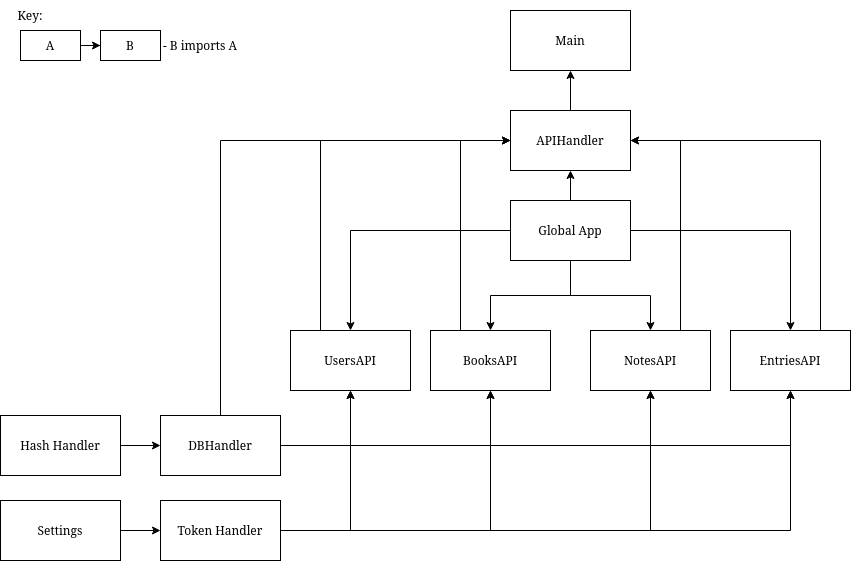
\includegraphics[width=0.9\linewidth]{Images/SSD-Backend-File-Structure.png}
    \caption{Python Import Structure}
    \label{fig:PythonImportStructure}
\end{figure}

\subsubsection{Overall Structure}

The application separates responsibilities into the frontend, backend, and the database. The frontend manages user interaction and preliminary validation, the backend enforces authorization, authentication, and input validation, and the database manages storage. This separation improves maintainability and ensures security is enforced server-side, preventing client-bypass vulnerabilities.  

\begin{figure}[h]
    \centering
    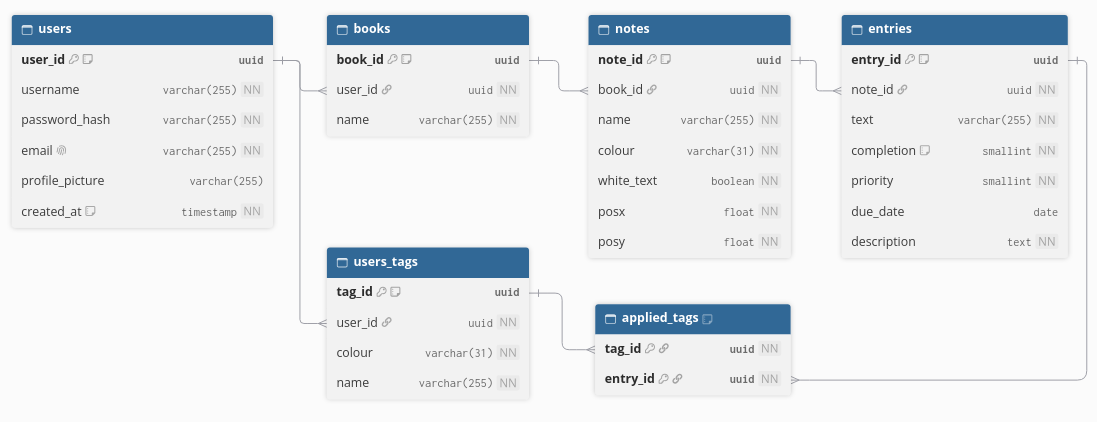
\includegraphics[width=0.9\linewidth]{Images/DbDesign.png}
    \caption{PostgreSQL Database Design.}
    \label{fig:DatabaseDesign}
\end{figure}


\subsubsection{How layers interact}

The frontend handles and validates user interaction before sending it to the REST API in the backend, which validates the JWT, ensuring the user is authenticated and authorised. It also validates the request, and sends it to the data management layer, where required queries are performed. Data then travels through the backend and back to the frontend, where it is displayed for the user. 



\subsection{Class Diagram}

\subsubsection{UML}
\begin{figure}[h]
    \centering
    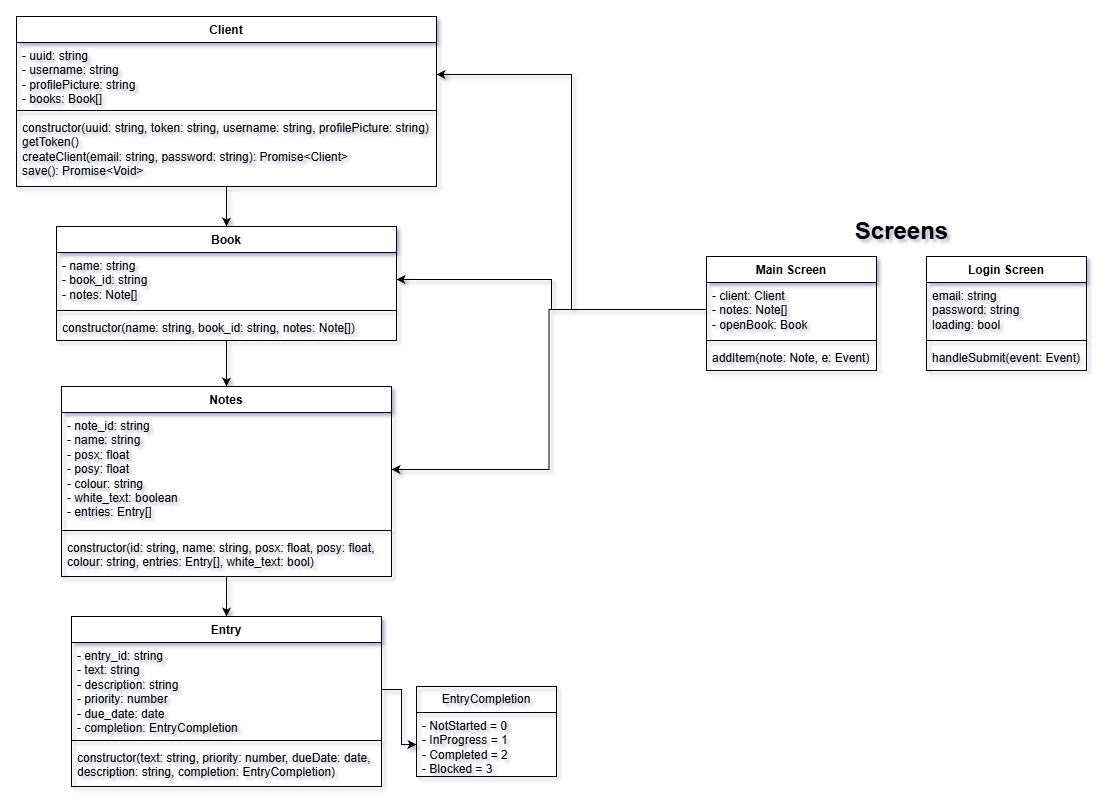
\includegraphics[width=1\linewidth]{Images/SSD_CW_UML.drawio.png}
    \caption{Frontend UML Diagram}
    \label{fig:FrontUML}
\end{figure}

\begin{figure}[h]
    \centering
    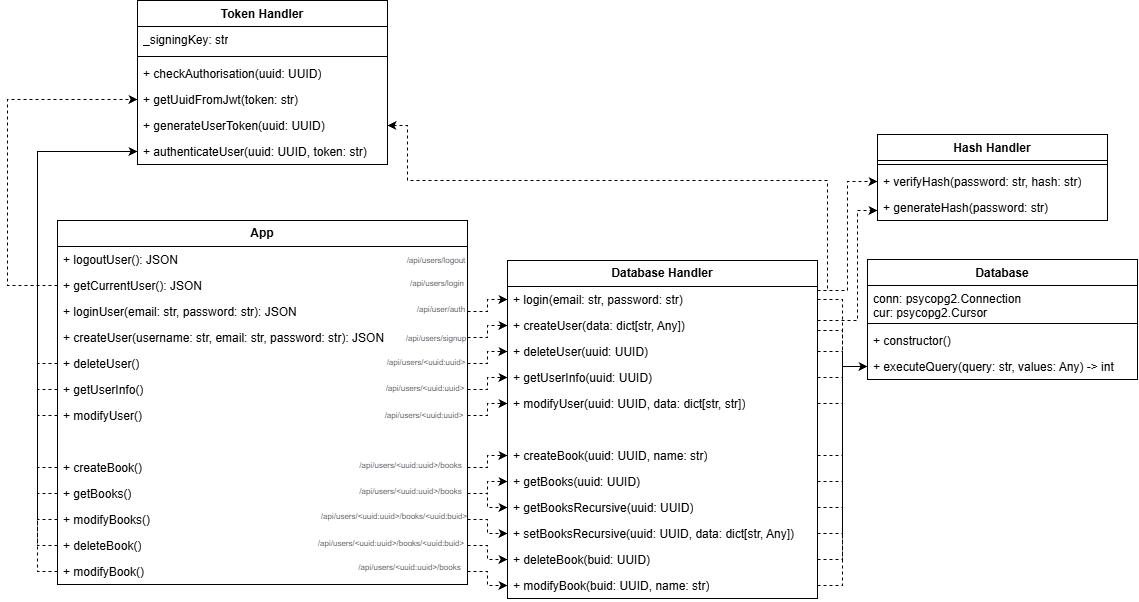
\includegraphics[width=1\linewidth]{Images/SSDBackendUML.png}
    \caption{Backend UML Diagram}
    \label{fig:BackUML}
\end{figure}
\newpage


\clearpage
\subsubsection{DFD and STRIDE}

\begin{figure}[h]
    \centering
    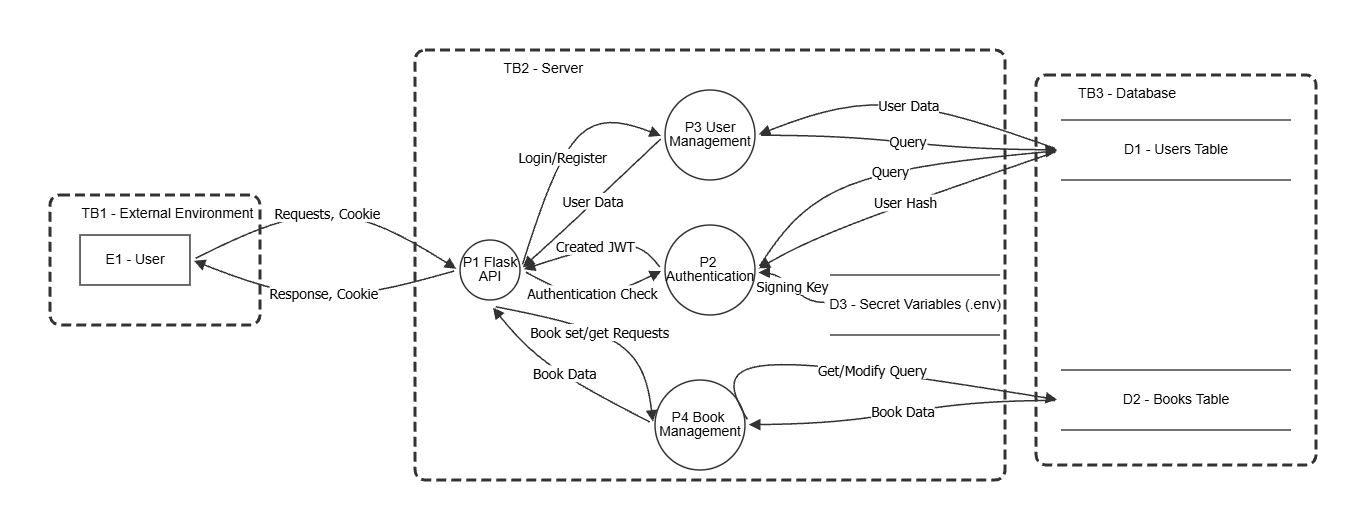
\includegraphics[width=1\linewidth]{Images/STRIDE Diagram.png}
    \caption{DFD Diagram}
    \label{fig:DFD}
\end{figure}

\begin{longtable}{|p{1.5cm}|p{4.5cm}|p{8cm}|}
     \hline

    \hline
    \textbf{ID} &
    \textbf{Name} & 
    \textbf{Description} \\ \hline
    \endhead

    TB1 & External Environment & The internet \\ \hline
    TB2 & Server & The server running the service \\ \hline
    TB3 & Database & The PostgreSQL database. \\ \hline
    


    E1 & User & User Client. \\ \hline
    
    P1 & Flask API & API handler. \\ \hline
    P2 & Authentication & Handles user authentication and token management. \\ \hline
    P3 & User Management & Handles Users. \\ \hline
    P4 & Book Management & Handles Books. \\ \hline
    
    D1 & Users Table & Contains user information. \\ \hline
    D2 & Books Table & Contains books. \\ \hline
    D3 & Secret Variables (.env) & Contains environment variables. \\ \hline

    \caption{DFD Elements}
    \label{tab:dfdElements}

\end{longtable}









\begin{longtable}{|p{2cm}|p{1.4cm}|p{5.6cm}|p{5cm}|}
    \hline

    \textbf{STRIDE Category} &
    \textbf{Affected ID} &
    \textbf{Threat} &
    \textbf{Mitigation} \\
    \hline
    \endfirsthead

    \hline
    \textbf{STRIDE Category} &
    \textbf{Affected IDs} &
    \textbf{Threat} &
    \textbf{Mitigation} \\
    \hline
    \endhead

    Spoofing & E1, P2 &
    Impersonation of a legitimate user via stolen or forged credentials &
    Ensure cookies are HTTP-Only, ensure JWTs are valid, ensure JWTs expire \\ \hline
    
    Tampering & P1 &
    Modification of requests to manipulate application behaviour &
    Validate users are authorised to access material. \\ \hline
    
    Tampering & E1 &
    Bypassing client side validation &
    Ensure authorisation occurs server side. \\ \hline
    
    Tampering & P3, D2 &
    Modification of user records to gain authorisation &
    Use minimal database permissions, use server side authorisation \\ \hline
    
    Tampering & P2 &
    Tampering with JWT contents to alter claims &
    Verify JWT signatures using secure algorithm \\ \hline
    
    Information Disclosure & P1 &
    Internal errors are exposed through API request &
    Return generic error messages. \\ \hline
    
    Information Disclosure & P2 &
    JWTs or credentials are exposed through insecure communication &
    Ensure HTTPS is enabled, use secure and HTTPOnly cookies. \\ \hline
    
    Information Disclosure & D3 &
    Environment variables accessed, containing secret information like signing keys &
    Exclude .env from git, use a secrets manager \\ \hline

    



    
    \caption{STRIDE Threat Assessment}
    \label{tab:stride}   
    
\end{longtable}






\subsubsection{Important classes}

In the frontend, Client stores user information such as books, tags, and their UUID. This also provides an abstraction layer between the TSX components and the API.

Frontend display is divided into two screens: Main and Login. Main handles app interactions and variables such as open book and notes. Login handles logging in and signing up, as well as Client creation.

The backend uses the Flask 'app' class to manage the API, and the database is handled by a 'database' class, which acts as an abstraction layer between the backend and the PostgreSQL database.








\subsection{Secure Design Principles}

\subsubsection{Least Privilege}

Least privilege ensures users have minimal privilege required to complete tasks, minimising attack surface, for example users only being able to access their own notes.

\subsubsection{Separation of concerns}

Separation of concerns divides complex problems into smaller, independent components with distinct responsibilities. This improves modularity and readability.

The application implements this in three layers: frontend, backend, and data management. With each having a separate purpose, changes cause minimal changes to other layers.

\subsubsection{Input validation}

Input validation occurs primarily in the backend, as frontend validation can be bypassed. However, frontend validation still occurs to reduce unnecessary server load.

Validation ensures data is correct and prevents malicious payloads, reducing the risk of injection vulnerabilities.

\subsubsection{Defence in depth}

Defence in depth uses multiple layers of security to reduce chances of a security breach, as bypassing one layer does not compromise the entire application.

This is implemented through backend authentication, authorisation, input validation rejecting invalid requests, and parametrised SQL queries preventing SQL injection. These measures prevent unauthorised access through many layers of security.